\section{Results}\label{sec:exp}

In the first part of this section, we describe the benchmark infrastructure and the
images we used for the measurements. Then we analyze how different compilers and flags
affect the performance of our code. In the end, we discuss each optimization and compare
them in different plots.

\mypar{Experimental setup} All benchmarks and tests were conducted on an Intel
Core i7-8650U processor with \textit{Intel Turbo Boost} disabled, running at 1.9
GHz. The CPU has a 4$\times$32 KB 8-way associative L1 cache, a 4$\times$256 KB
4-way associative L2 cache and 4$\times$2 MB 16-way associative L3 cache
\cite{intel-opt-manual}.

We used the peak signal-to-noise ratio (PSNR) to ensure that our baseline implementation
compresses the image correctly. This metric is widely applied to compare an image with its
compressed version. Typical values for the PSNR range from 25 to
50 dB (higher is better). The same metric was used to verify that the optimizations
produced the same result as the baseline.

The PSNR of the compressed image depends on the maximum depth $m$ of the quadtree and the error
threshold $\epsilon$. We set $m=7$ and $\epsilon=300$ for all our experiments. These parameters
produced an image of good quality in a reasonable amount of time.

We chose to benchmark our algorithm with a challenging image depicting a lioness
with its cub \cite{lions}.
While some parts of the image, for example the
background, are easy to compress, other parts such as the fur contain lots of details,
which are harder to compress. Figure \ref{fig:lions} shows the output of the
vectorized code with $\epsilon=100$ and 3 decompression iterations.

\begin{figure}[H]
  \centering
  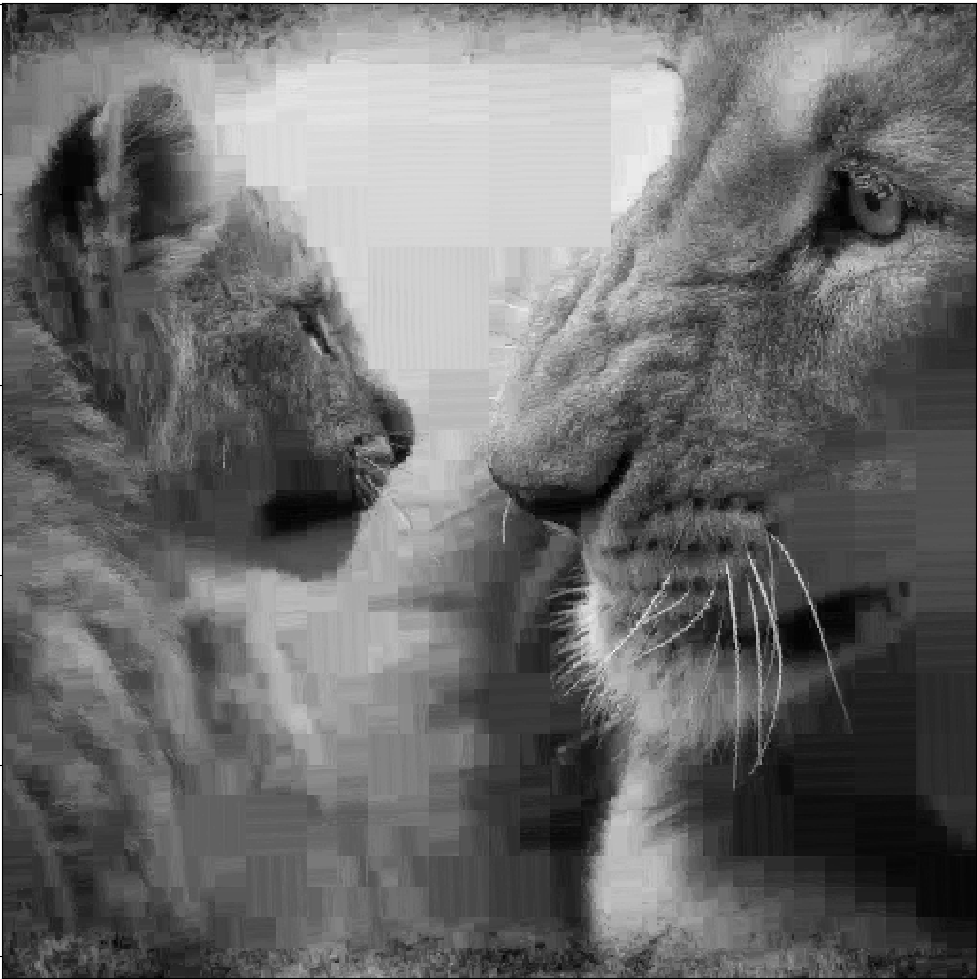
\includegraphics[page=1, width=.45\textwidth]{lion_512_51_e100}
  \caption{Decompressed Image}\label{fig:lions}
\end{figure}

\mypar{Compiler Flags} Several benchmarks were conducted comparing the achieved
performance using different compiler flags for the \textit{GNU Compiler
  Collection (gcc)} version 9.3.0 and the \textit{Intel C++ Compiler (icc)}
version 19.1.1.217. For all tests \texttt{-march=native} was set.

For both the scalar and the vectorized versions the flag \texttt{-O1} increased
performance significantly. While \texttt{-O2} did improve the scalar
implementation (figure \ref{fig:perf_scal}), it did not make a difference for
the vectorized version (figure \ref{fig:perf_vec}). Neither \texttt{-O3} nor
\texttt{-Ofast} were able increase performance for both code versions.

\begin{figure}[H]
  \centering
  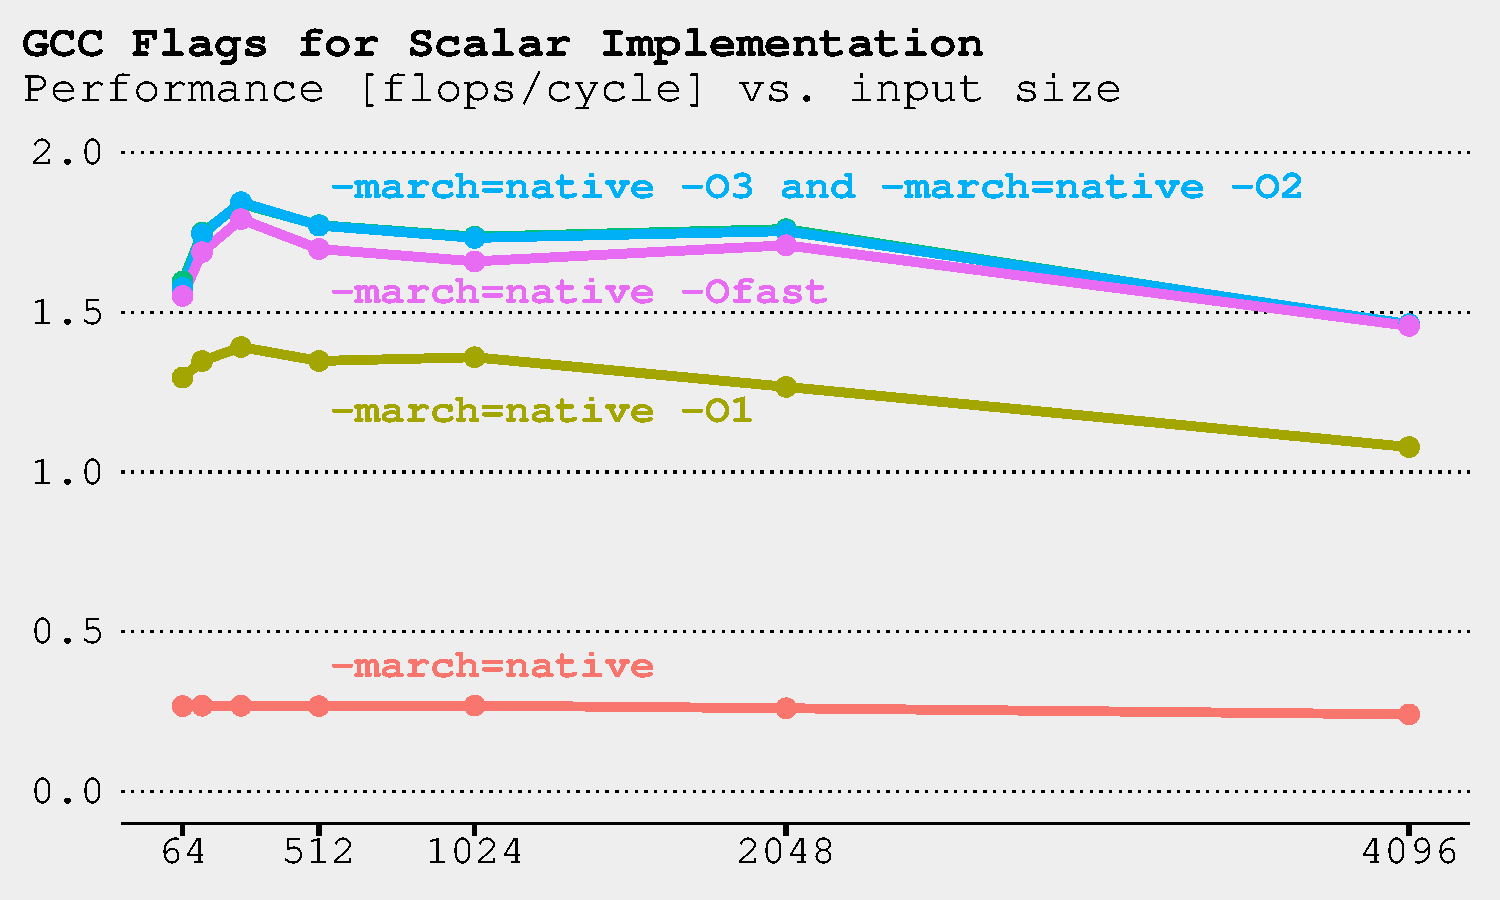
\includegraphics[page=1, width=\linewidth]{performance_scalar_opts}
  \caption{Performance of the four major GCC optimization flags for the scalar
    implementation}\label{fig:perf_scal}
\end{figure}

\begin{figure}[H]
  \centering
  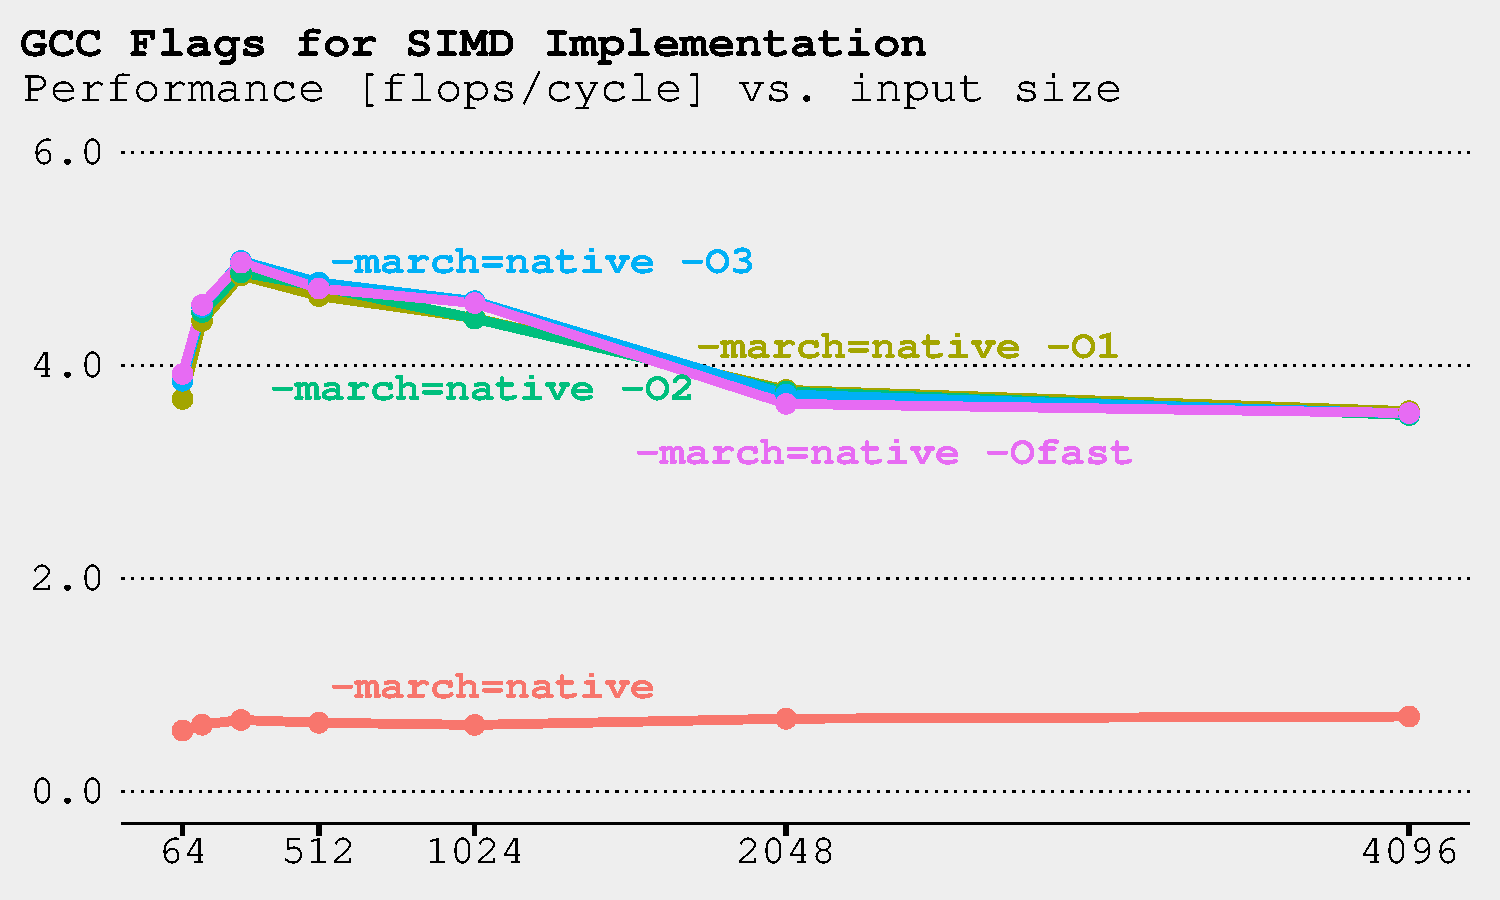
\includegraphics[page=1, width=\linewidth]{performance_vectorized_opts}
  \caption{Performance of the four major GCC optimization flags for the vectorized implementation}\label{fig:perf_vec}
\end{figure}

Intel's compiler was not able to outperform gcc but at least for the vectorized
version it managed to keep up for the larger images as shown in figure
\ref{fig:perf_gcc_vs_icc}.

\begin{figure}[H]
  \centering
  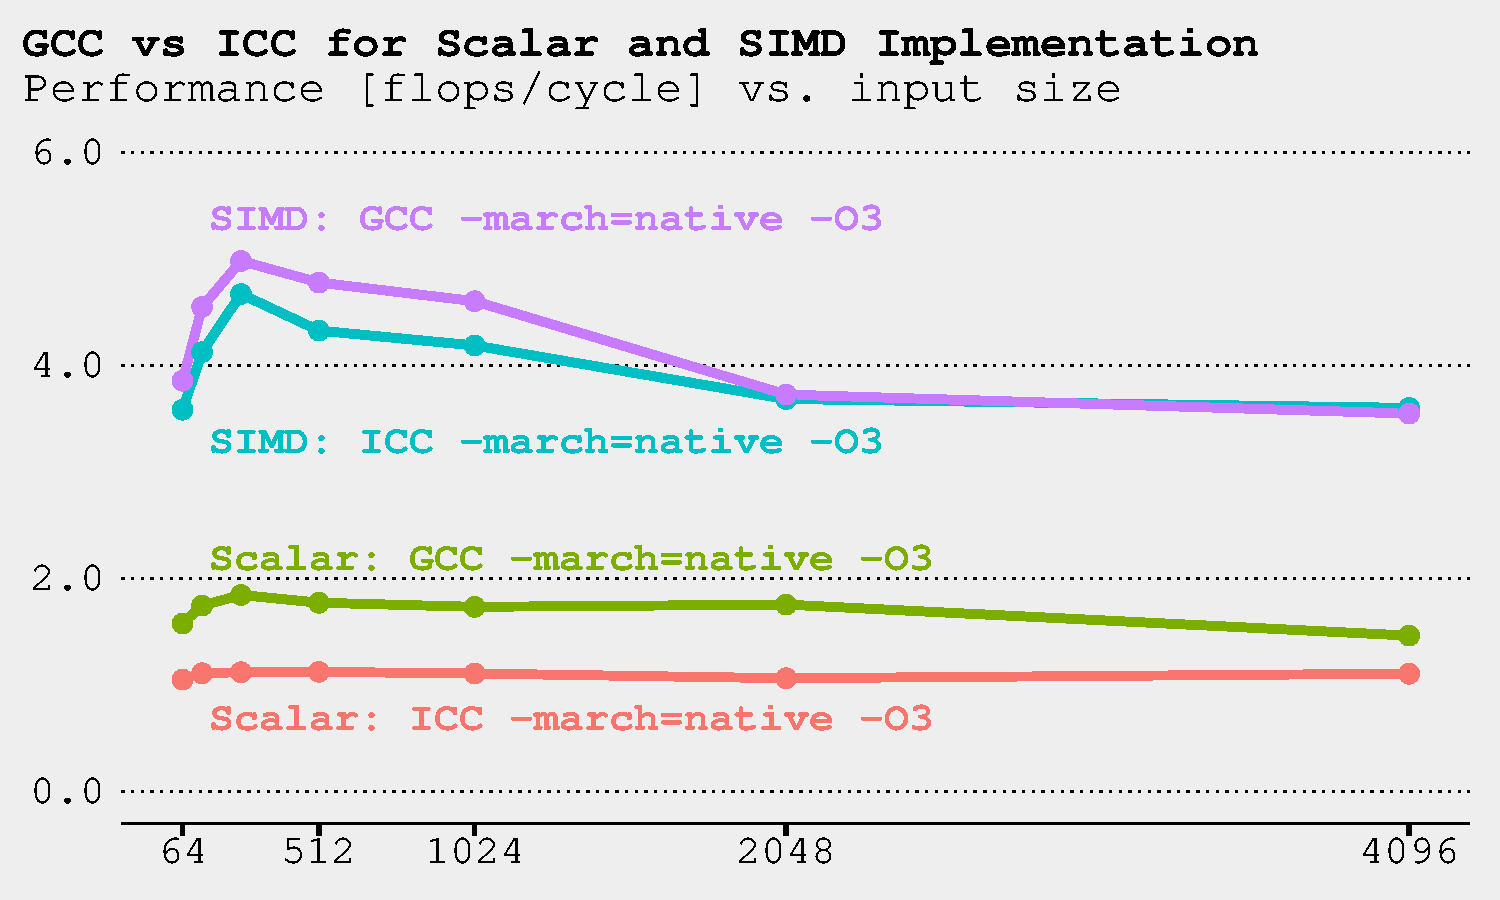
\includegraphics[page=1, width=\linewidth]{performance_gcc_vs_icc}
  \caption{Performance comparison between GCC and ICC with the best scalar and
    SIMD implementation}\label{fig:perf_gcc_vs_icc}
\end{figure}

Because the Intel compiler with various compiler flags did not lead to
improvements, we used gcc with the flags \texttt{-march=native -O3} which
performed best for all the upcoming benchmarks.

\mypar{Performance} The plot in figure~\ref{fig:perf} shows the performance of
our major implementations. As a first result we observe that our baseline
implementation achieves an equal or slightly better performance than the
open-source reference C\texttt{++} implementation~\cite{github-cpp}. Values for
large images are not shown in the plot because the measurements took too much
time.

The optimized scalar implementation which includes precomputations, a better
memory layout and ILP is four times faster than the baseline. The optimizations
become even more apparent when we compare the runtime as in figure
\ref{fig:runtime}. The plot shows that the runtime decreased by several orders
of magnitude and we were finally able to compress larger images in a reasonable
amount of time.

\begin{figure}[H]
  \centering
  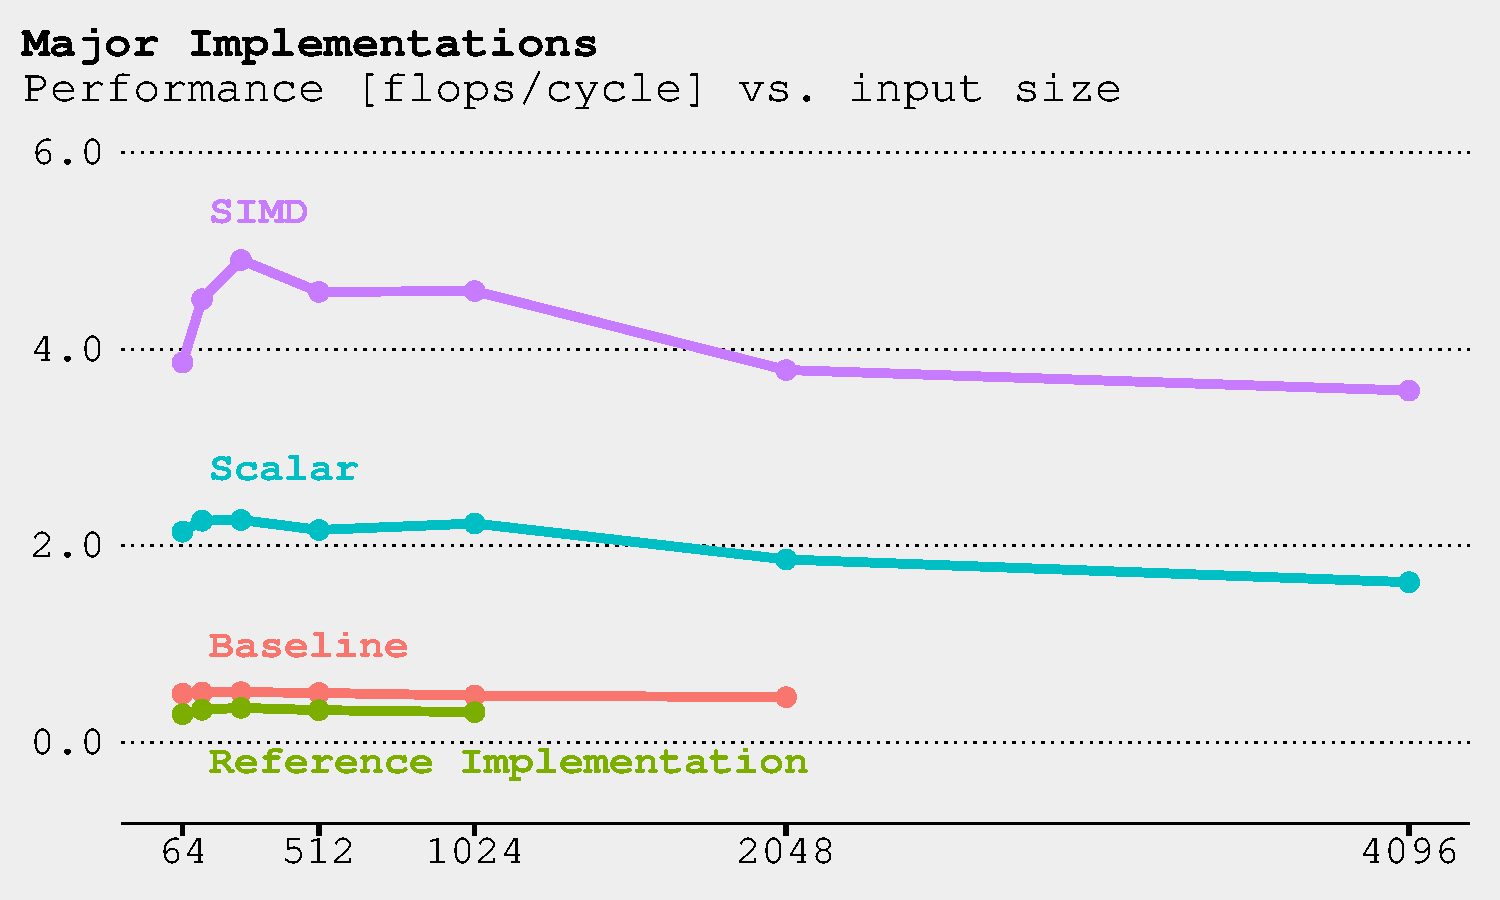
\includegraphics[page=1, width=\linewidth]{performance_major_versions}
  \caption{Performance of our three major implementations and a reference
    implementation from GitHub written in C\texttt{++}}\label{fig:perf}
\end{figure}


\begin{figure}[H]
  \centering
  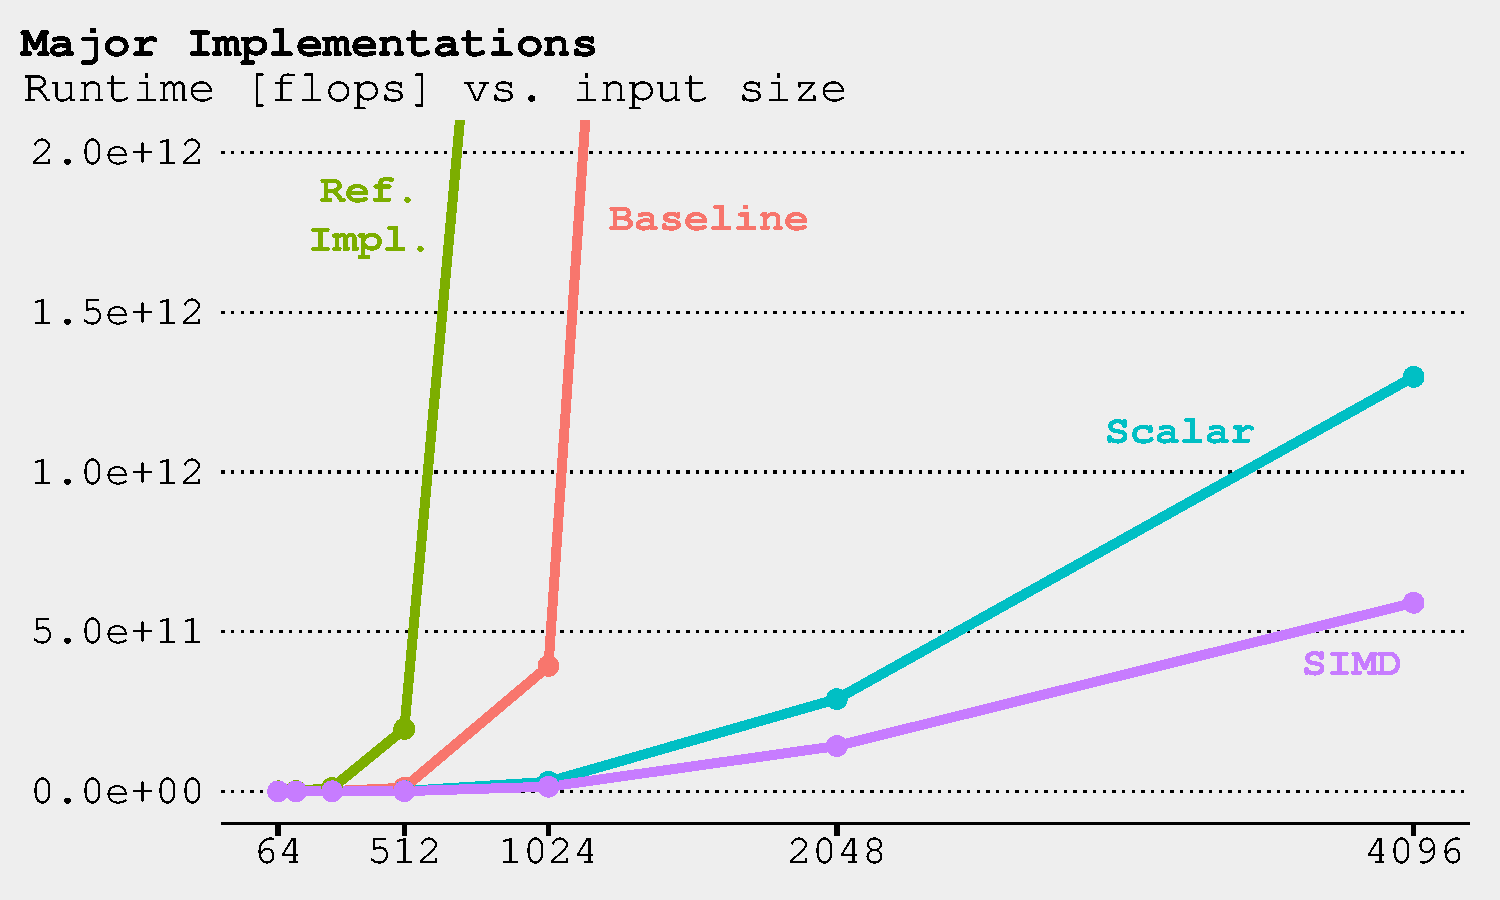
\includegraphics[page=1, width=\linewidth]{runtime_major_versions}
  \caption{Runtime of our three major implementations and a reference
    implementation from GitHub written in C\texttt{++}}\label{fig:runtime}
\end{figure}

As described in section \ref{sec:yourmethod} the initial attempt in vectorizing
the code did not lead to the expected performance improvements. In fact, it
performed just slightly better than the scalar optimized code. We suspected that
the gathering instructions, which are necessary for the rotations, are
responsible for poor performance. To verify this assumption, we removed the
column-wise access to the image i.e. 90/270 degree rotations from the scalar
optimized and the vectorized version. The result of this experiment is shown in
figure \ref{fig:perf_40_41} and one can clearly see how the vectorized code
outperforms the scalar optimized version.

\begin{figure}[H]
  \centering
  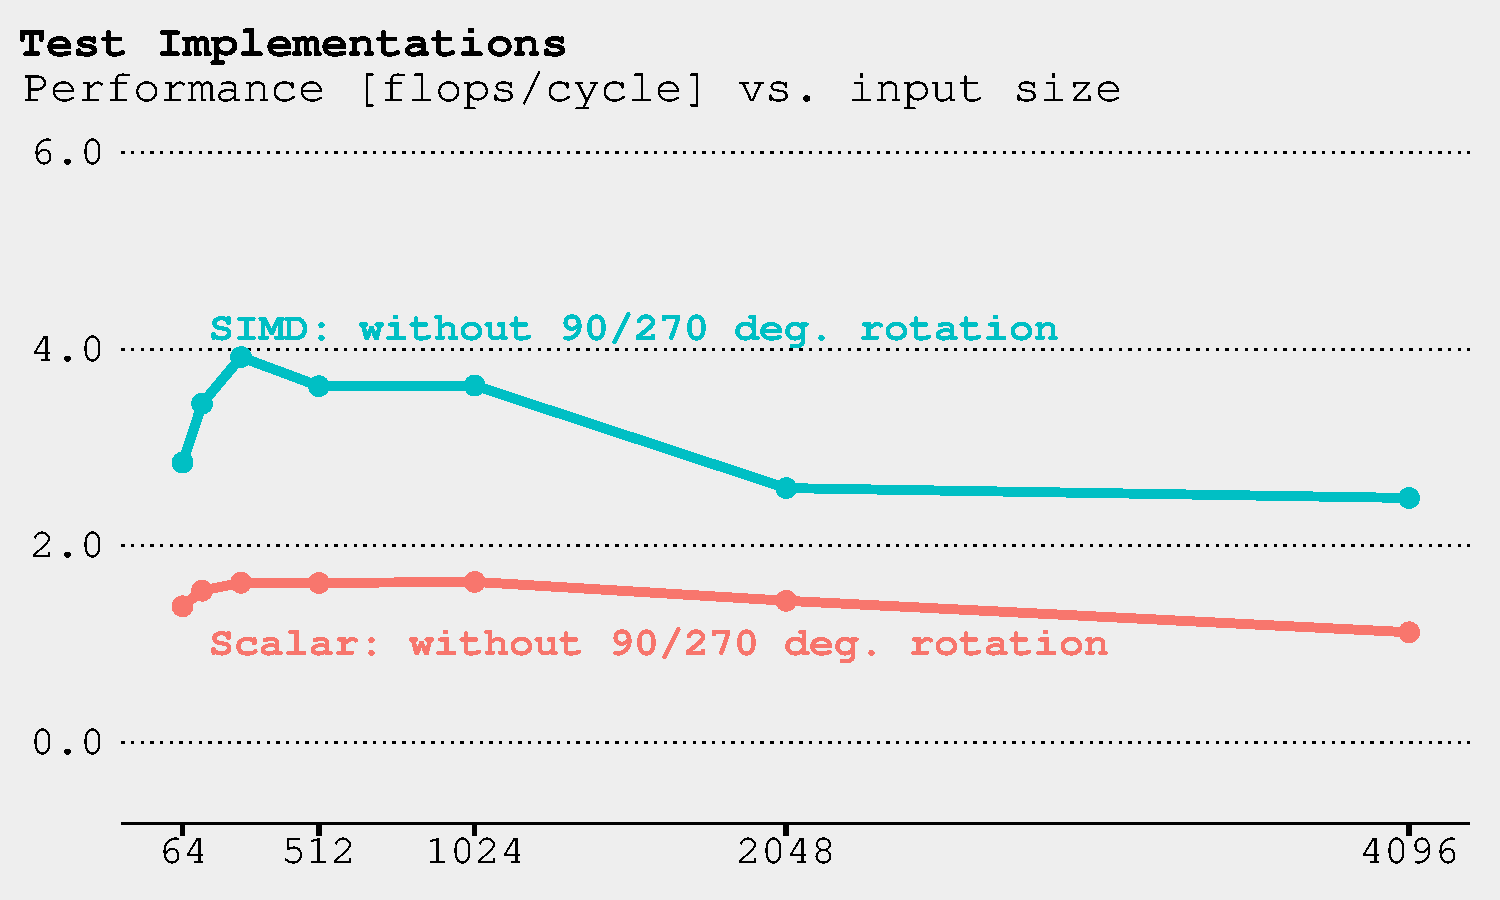
\includegraphics[page=1, width=\linewidth]{performance_norot}
  \caption{Performance Plot without 90/270 degree rotations}\label{fig:perf_40_41}
\end{figure}


After this experiment, we improved the column-wise access by rotating the range
block instead of the domain block for the 90/270 degree rotations. The improved
vectorized implementation has a performance roughly eight times as high as the
baseline and about twice the performance of the scalar optimized version. The
runtime was also reduced especially for large images.
